\section{Benchmarking of Planners}
In the previous sections, we found out the path plans for optimal welding using the 2Dof rotary table. We also addressed the problem of reachability and showed how it can be overcome using the table. In this chapter we will delve into the effects that the table has on the motion planners, in terms of time taken to generate a plan, correctness of solution generated and memory consumed while doing so. We consider 2 different scenarios, for benchmarking the planners first without optimizing the table position and next with the table optimization turned on. The following criteria were considered for comparing the results of the two use cases. The criteria are defined in \citet{moll2015benchmarking-motion-planning-algorithms}:
\begin{itemize}
	\item Time of Planning
	\item Status of Plans Generated
	\item Best Cost of Plans Generated
	\item Graph States: Number of samples generated by the planner during planning.
\end{itemize}
The use cases are illustrated in figures (\ref{bm:uc1} and \ref{bm:uc2}).
The configuration details of the planners are presented in the appendix section.
\begin{figure}[!htbp] %  figure placement: here, top, bottom, or page
	\centering
	\begin{subfigure}[b]{0.4\textwidth}
		\frame{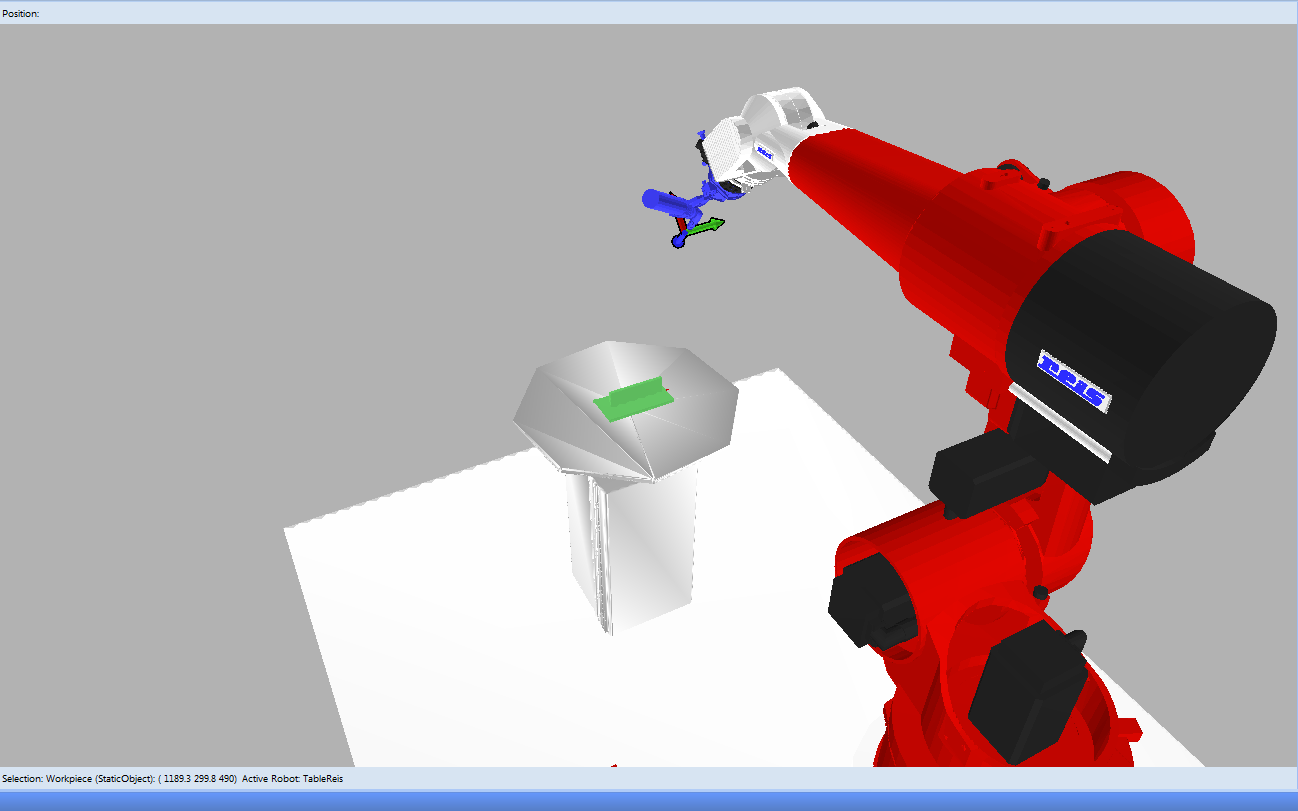
\includegraphics[width=1\textwidth,height=0.2\textheight]{images/un_opt_bnch.png}}
		\caption{Use Case Without Table Position Optimization}  
		\label{bm:uc1}
	\end{subfigure}
	\begin{subfigure}[b]{0.4\textwidth}
		\frame{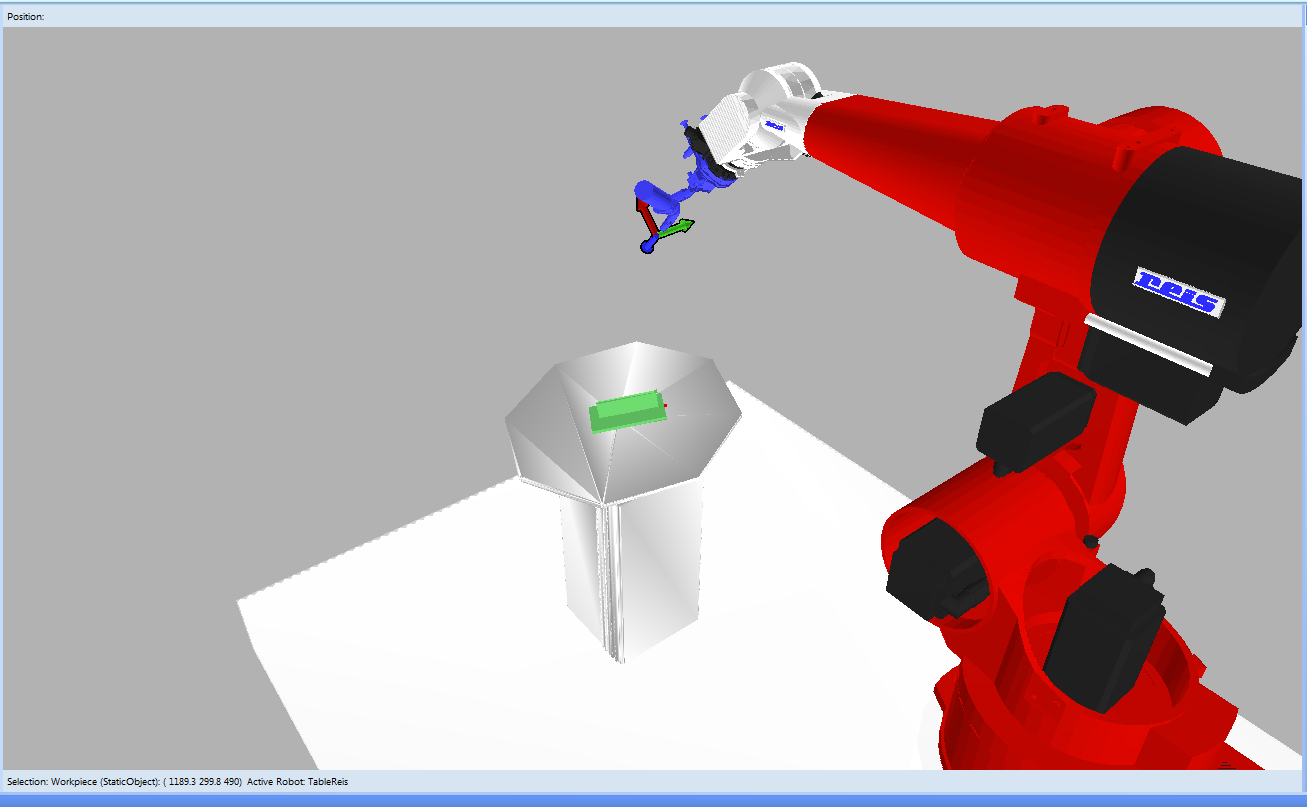
\includegraphics[width=1\textwidth,height=0.2\textheight]{images/opt_bnch.png}}
		\caption{Use Case With Table Position Optimization}  
		\label{bm:uc2}
	\end{subfigure}	
	\caption{Benchmarking Use Cases}
	\label{bm:uc}
\end{figure}
\clearpage
\begin{figure}[!htbp] %  figure placement: here, top, bottom, or page
	\centering
	\begin{subfigure}[b]{0.4\textwidth}
		\frame{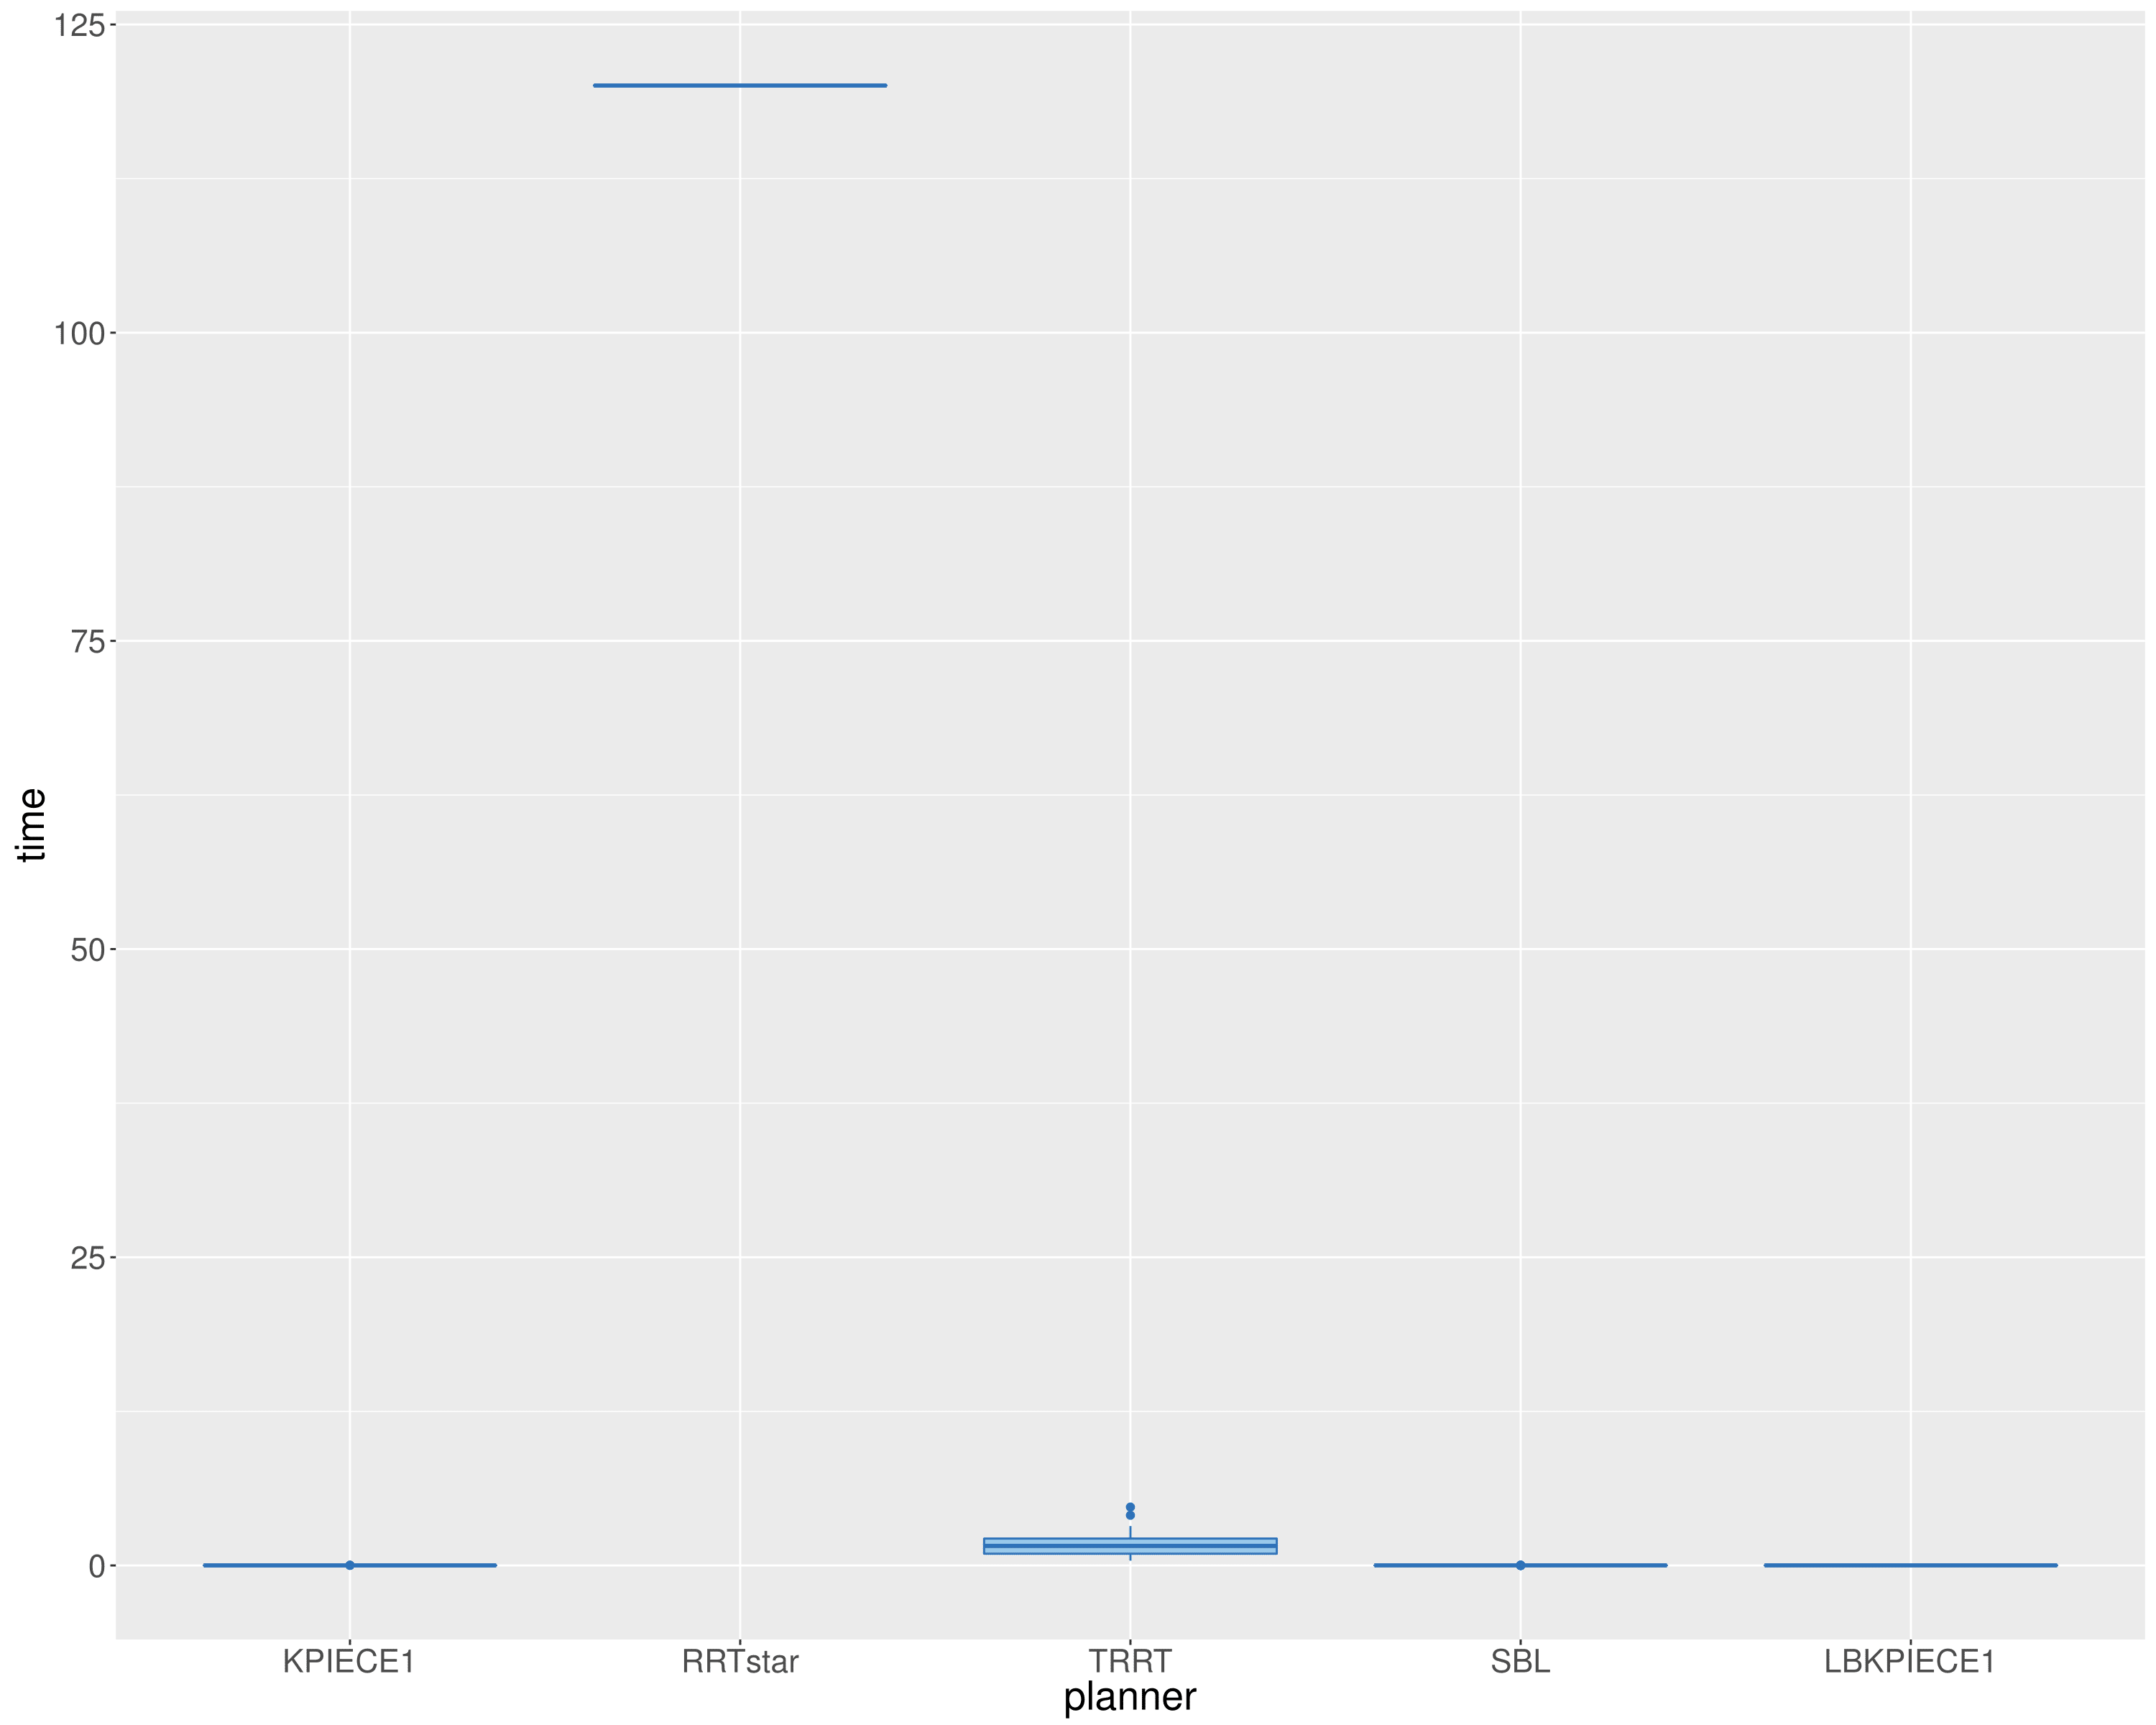
\includegraphics[width=1\textwidth,height=0.2\textheight]{images/opt_time-1.png}}
		\caption{Time Consumed for Unoptimized Motion Planning }
		\label{fig:bm1tu}
	\end{subfigure}
	\begin{subfigure}[b]{0.4\textwidth}
		\frame{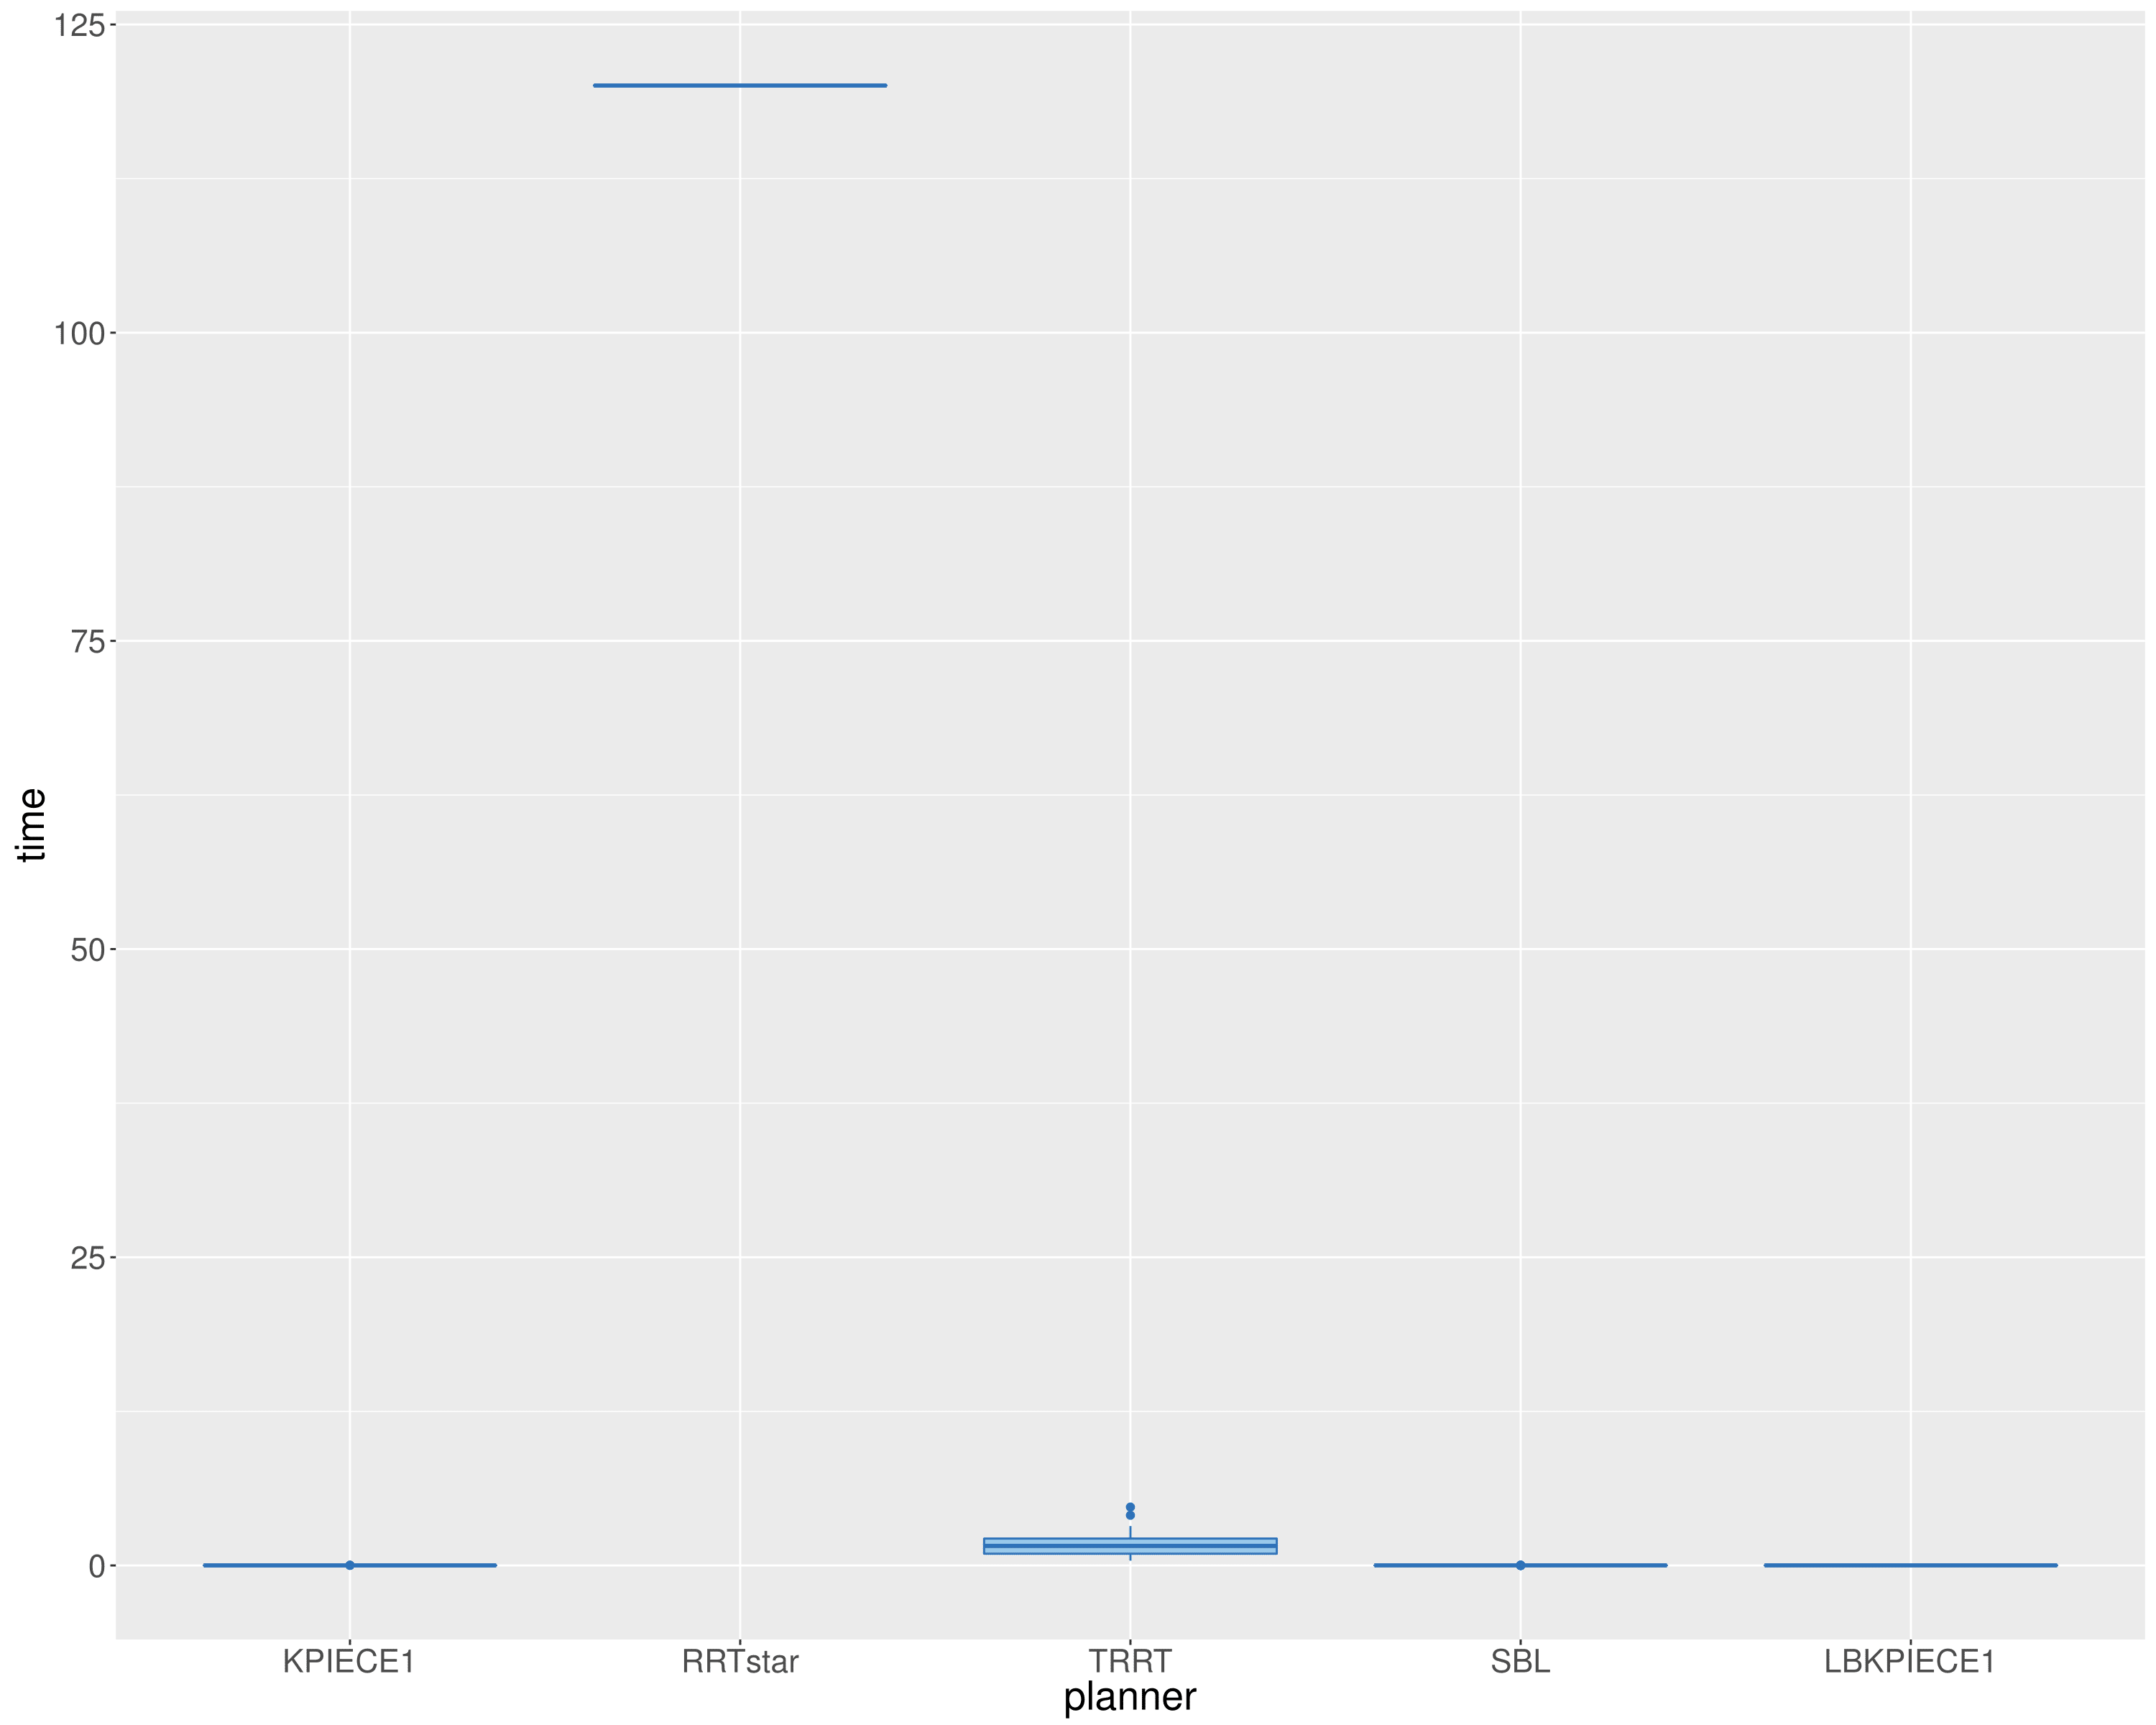
\includegraphics[width=1\textwidth,height=0.2\textheight]{images/opt_time-1.png}}
		\caption{Time Consumed for Optimized Motion Planning with Table}  
		\label{fig:bm1to}
	\end{subfigure}	
	\caption{Time Consumed for Motion Planning}
	\label{fig:bmt}
\end{figure}

In plot \ref{fig:bmt}, the time consumed by each planner for generating a successful plan is plotted. We can observe that the time taken by the planners in both cases are nearly identical. According to \citet{moll2015benchmarking-motion-planning-algorithms}, RRTstar takes almost the entire time allocated to it to generate plan because, it utilizes the time to optimize the solution it generates.

\begin{figure}[!htbp] %  figure placement: here, top, bottom, or page
	\centering
	\begin{subfigure}[b]{0.4\textwidth}
		\frame{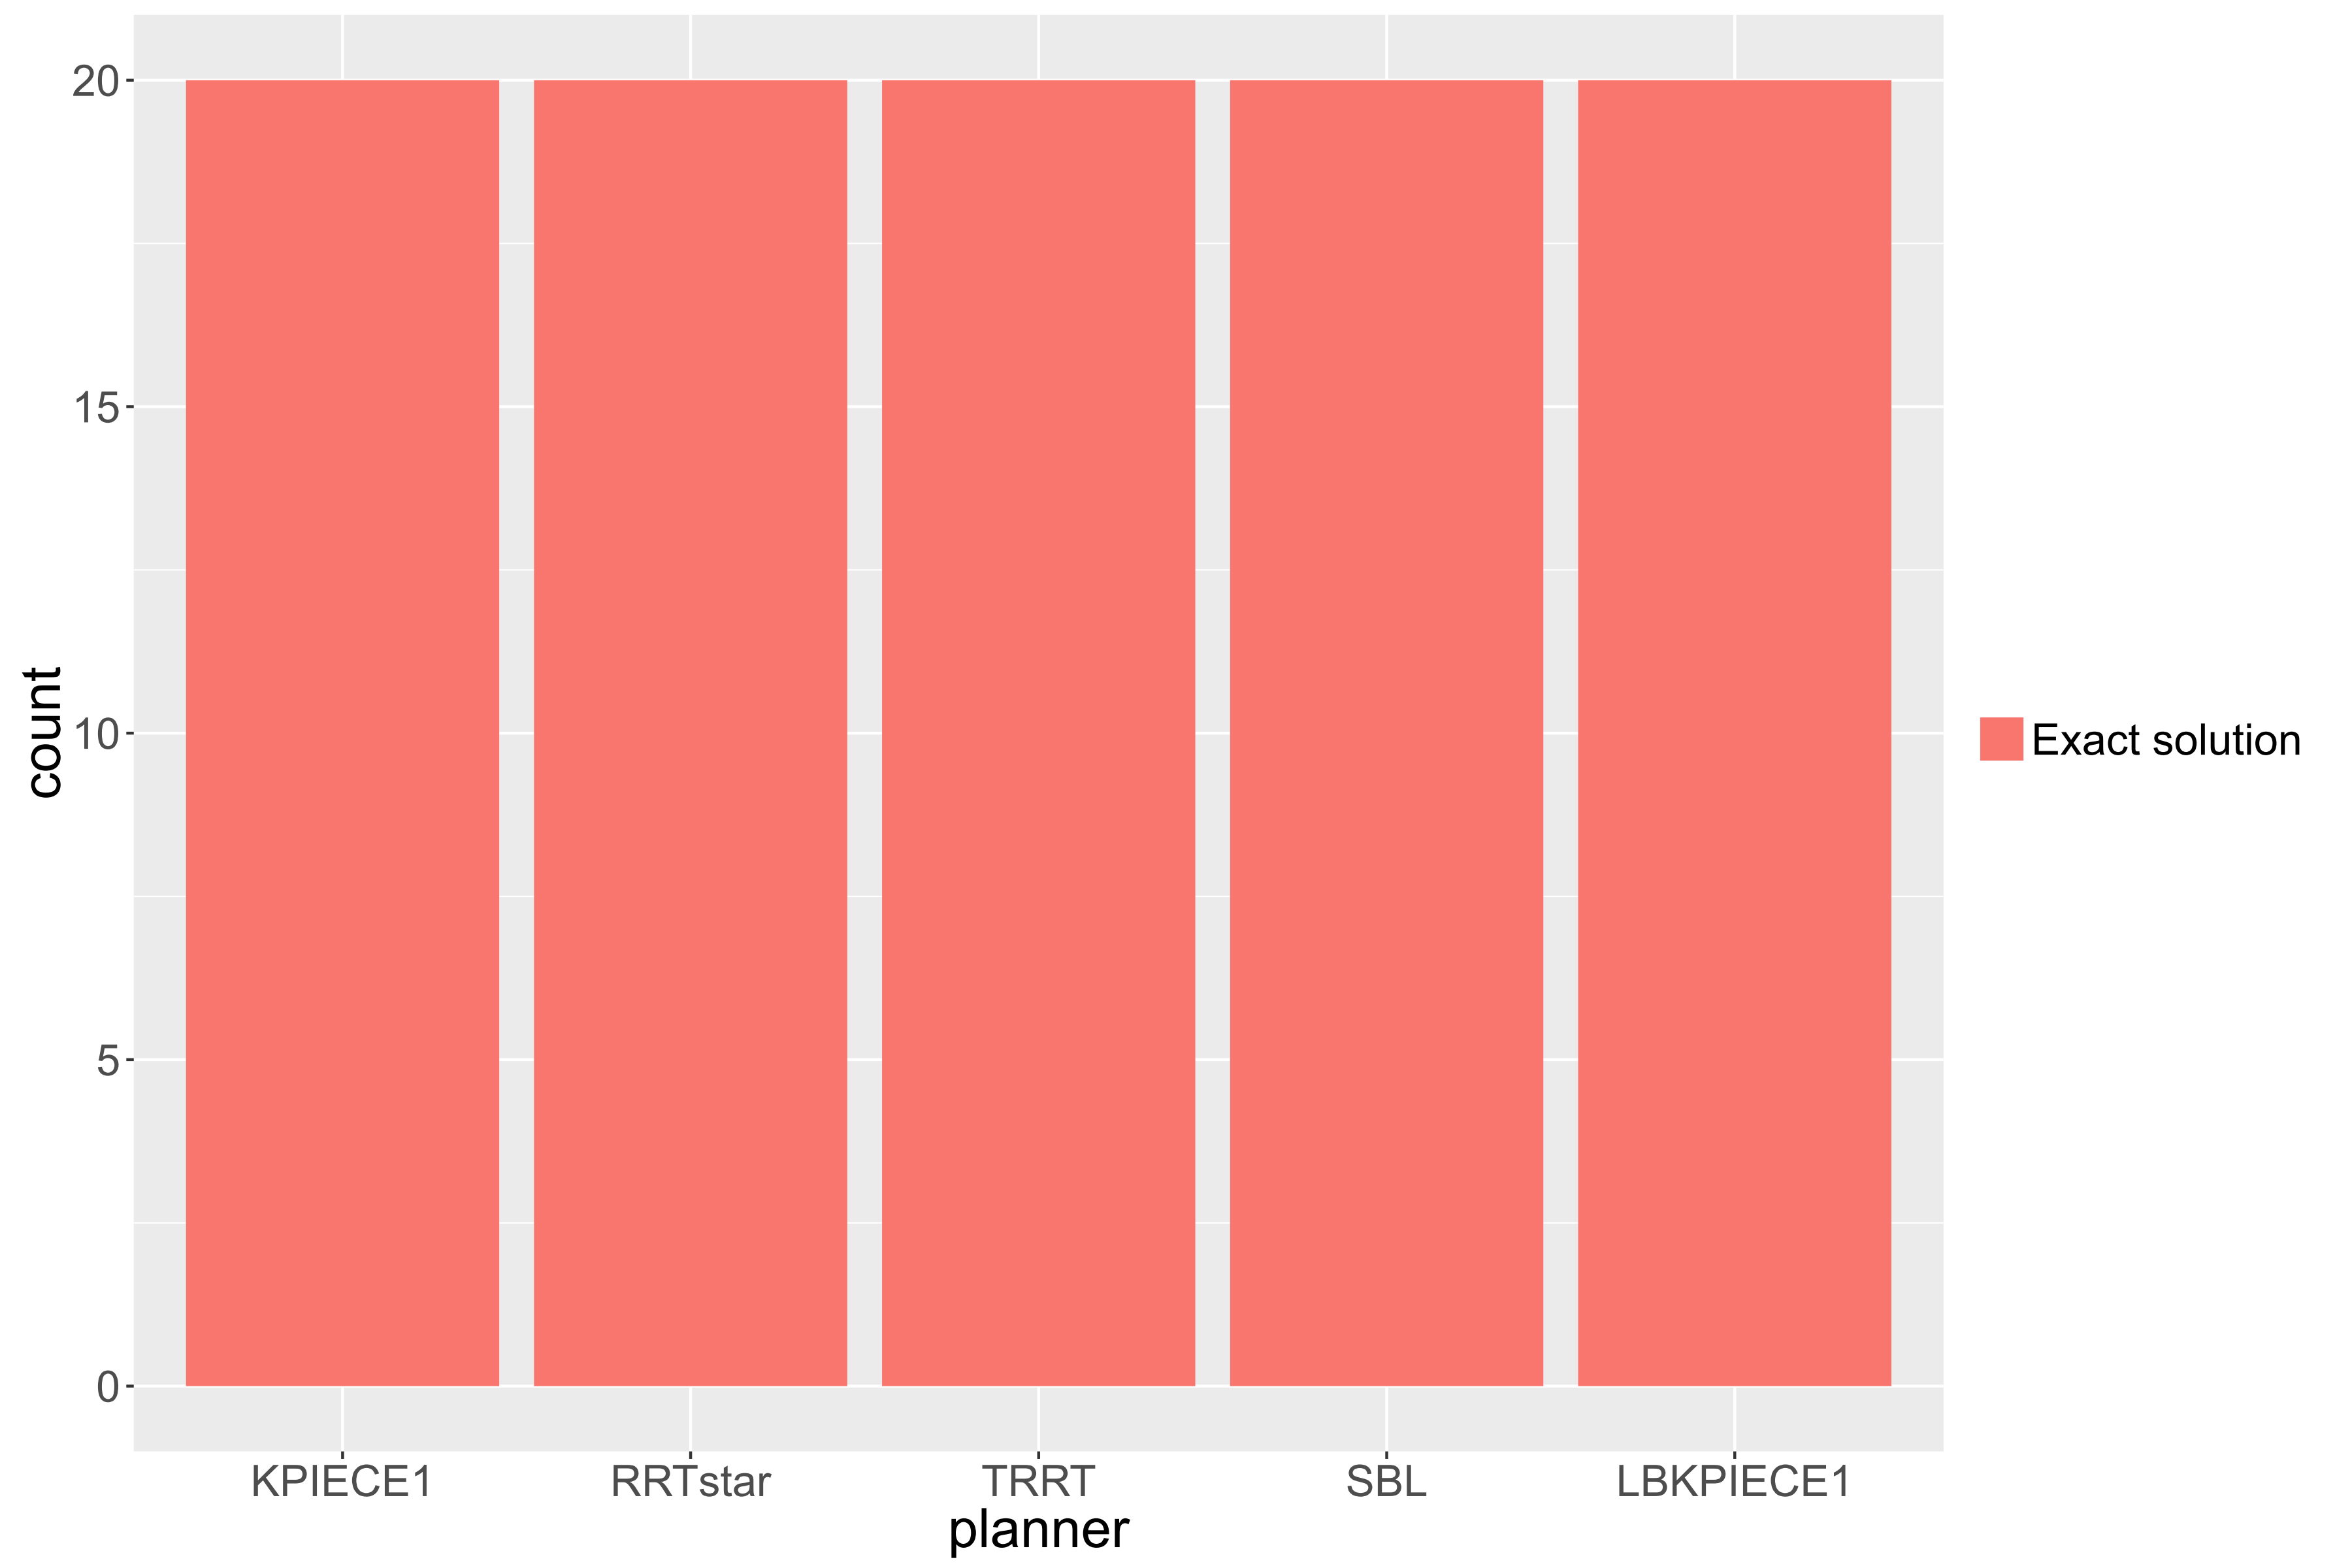
\includegraphics[width=0.8\textwidth,scale=0.6]{images/status_uopt.png}}
		\caption{Status of Motion Planning: Unoptimized}
		\label{fig:bms1}
	\end{subfigure}
	\begin{subfigure}[b]{0.4\textwidth}
		\frame{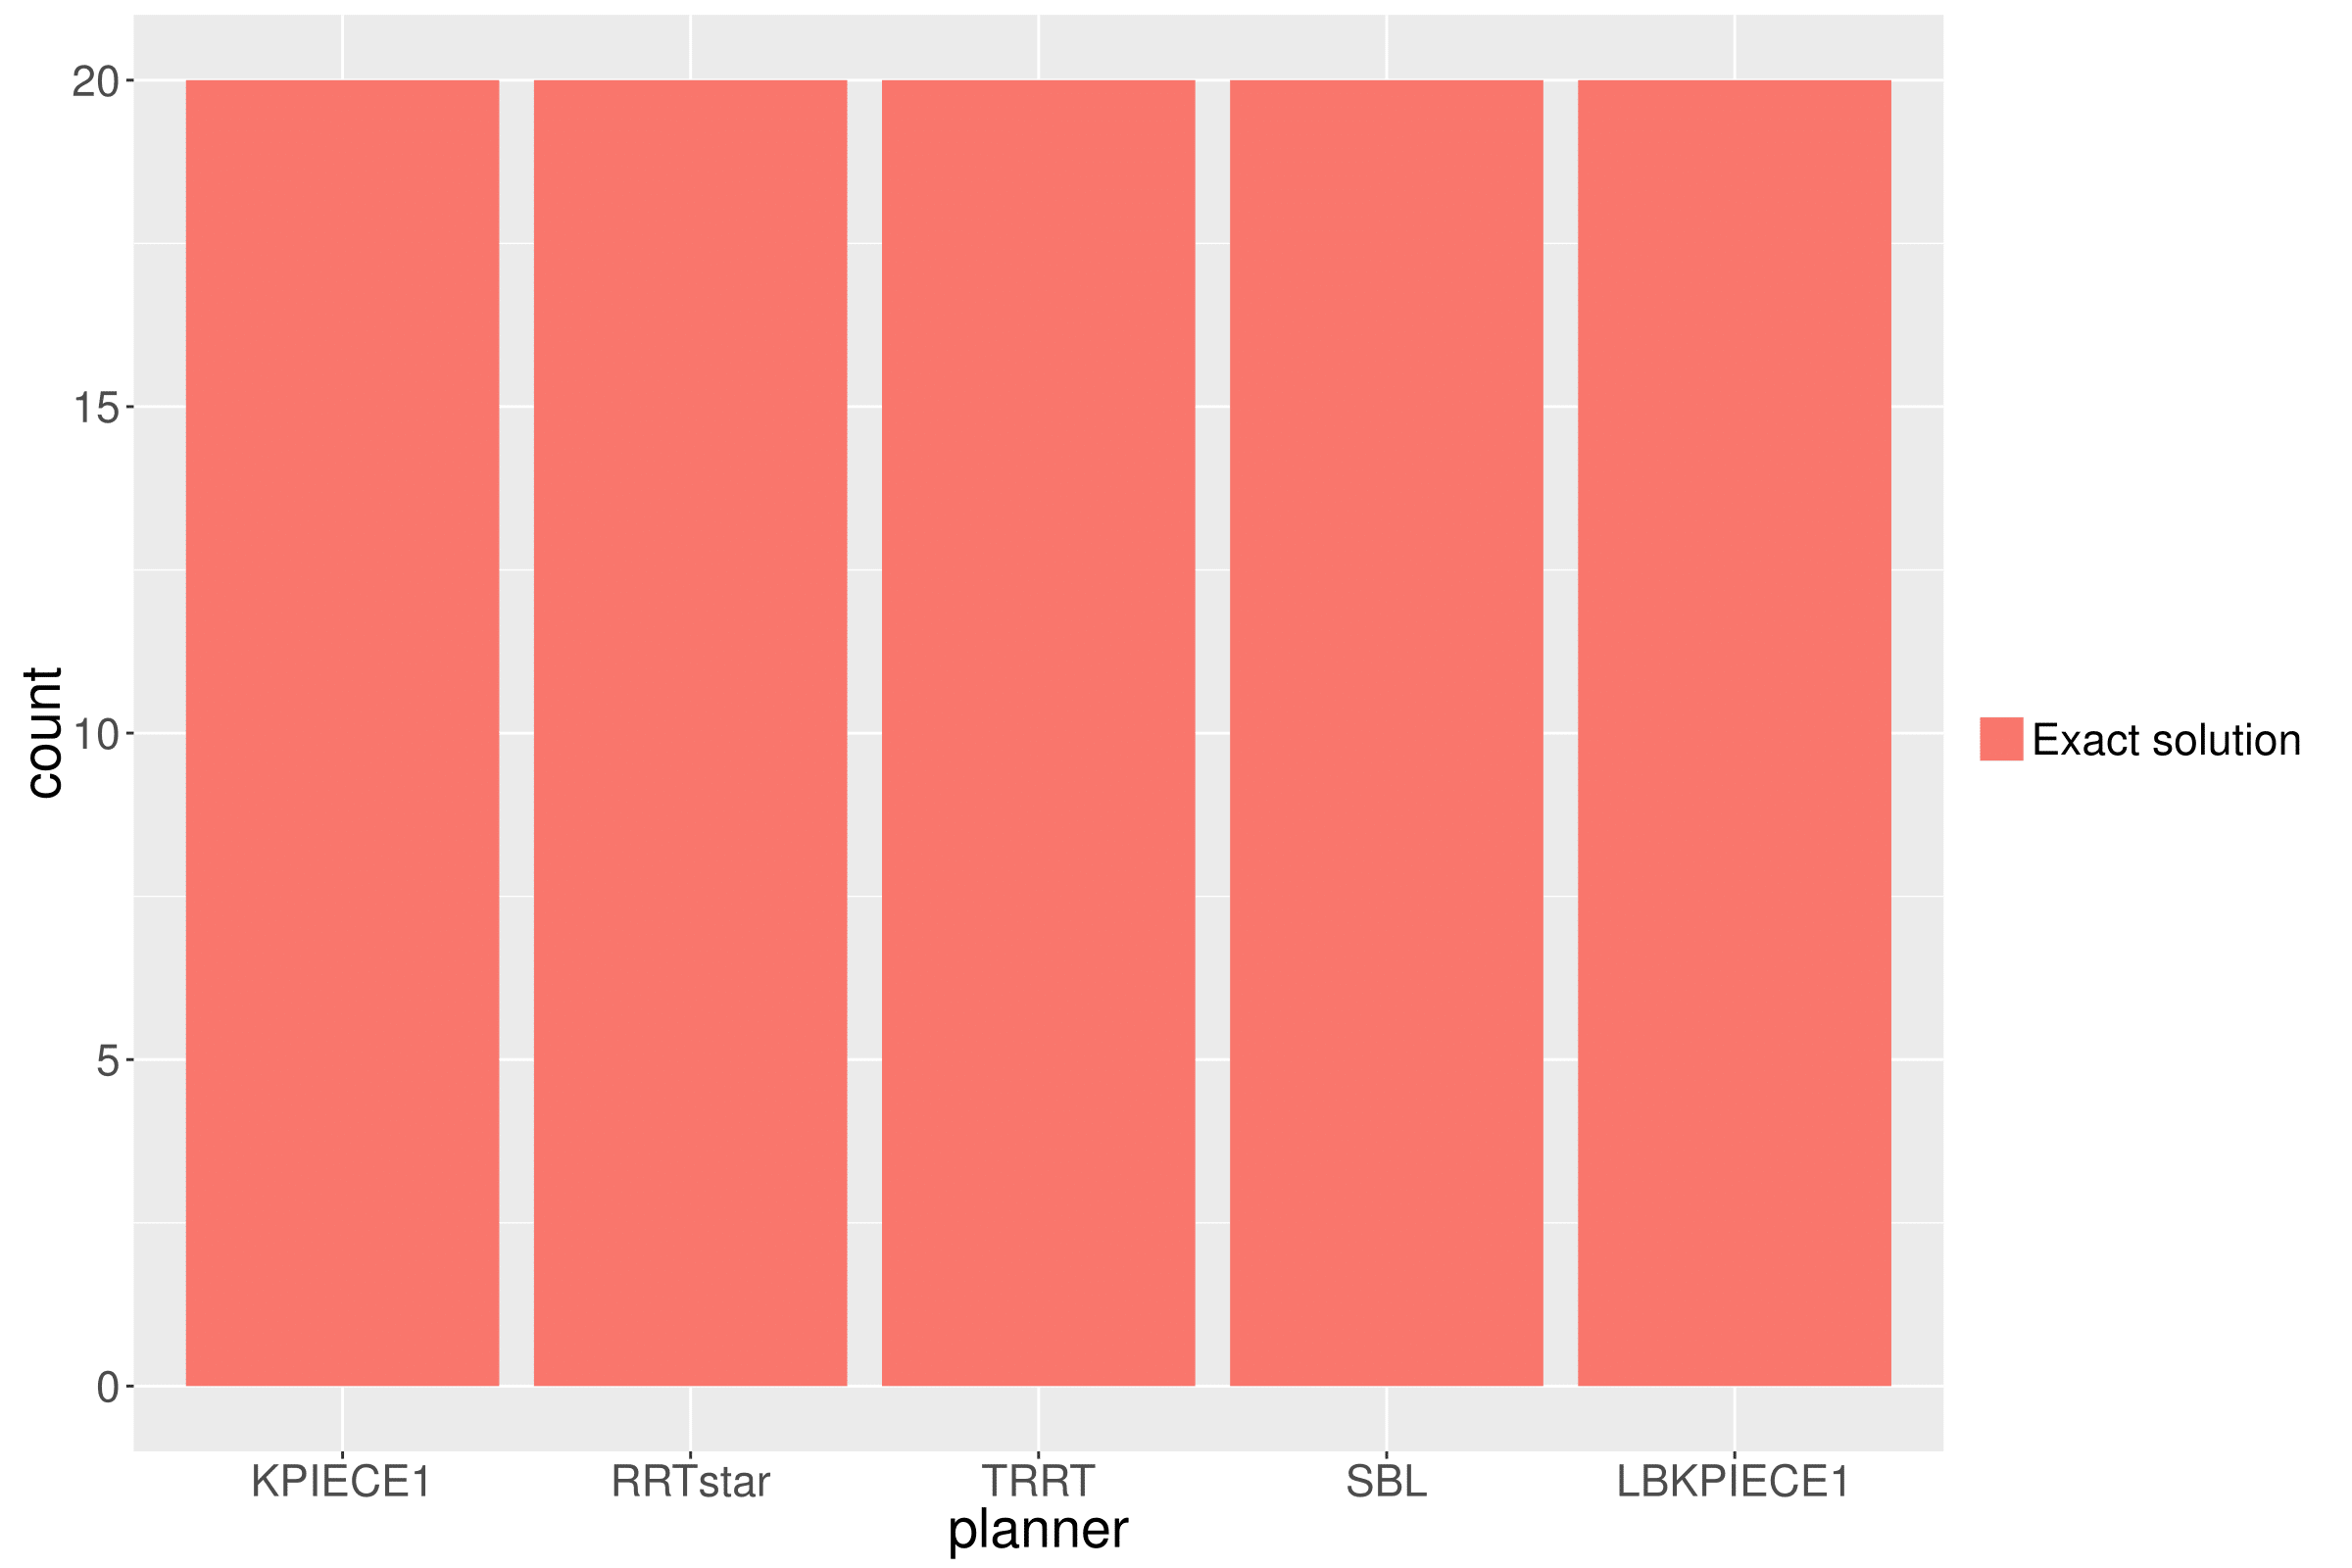
\includegraphics[width=0.8\textwidth,scale=0.6]{images/status_opt.png}}
		\caption{Status of Motion Planning:Using Table Optimization}
		\label{fig:bms2}
	\end{subfigure}	
	\caption{Status of Motion Planning:Using Table Optimization}
	\label{fig:bms}
\end{figure}
In plot \ref{fig:bms}, we can observe that the all the planners in both use cases are able to successfully solve the planning problem for every iterations. 

A key measure of a planner's performance is the, how much cost optimization it can perform, \citet{sucan2012the-open-motion-planning-library}. The benchmarking library currently records the best cost found only for the RRTstar, so the data for RRTstar is presented in figure 

\begin{figure}[!htbp] %  figure placement: here, top, bottom, or page
	\centering
	\begin{subfigure}[b]{0.4\textwidth}
		\frame{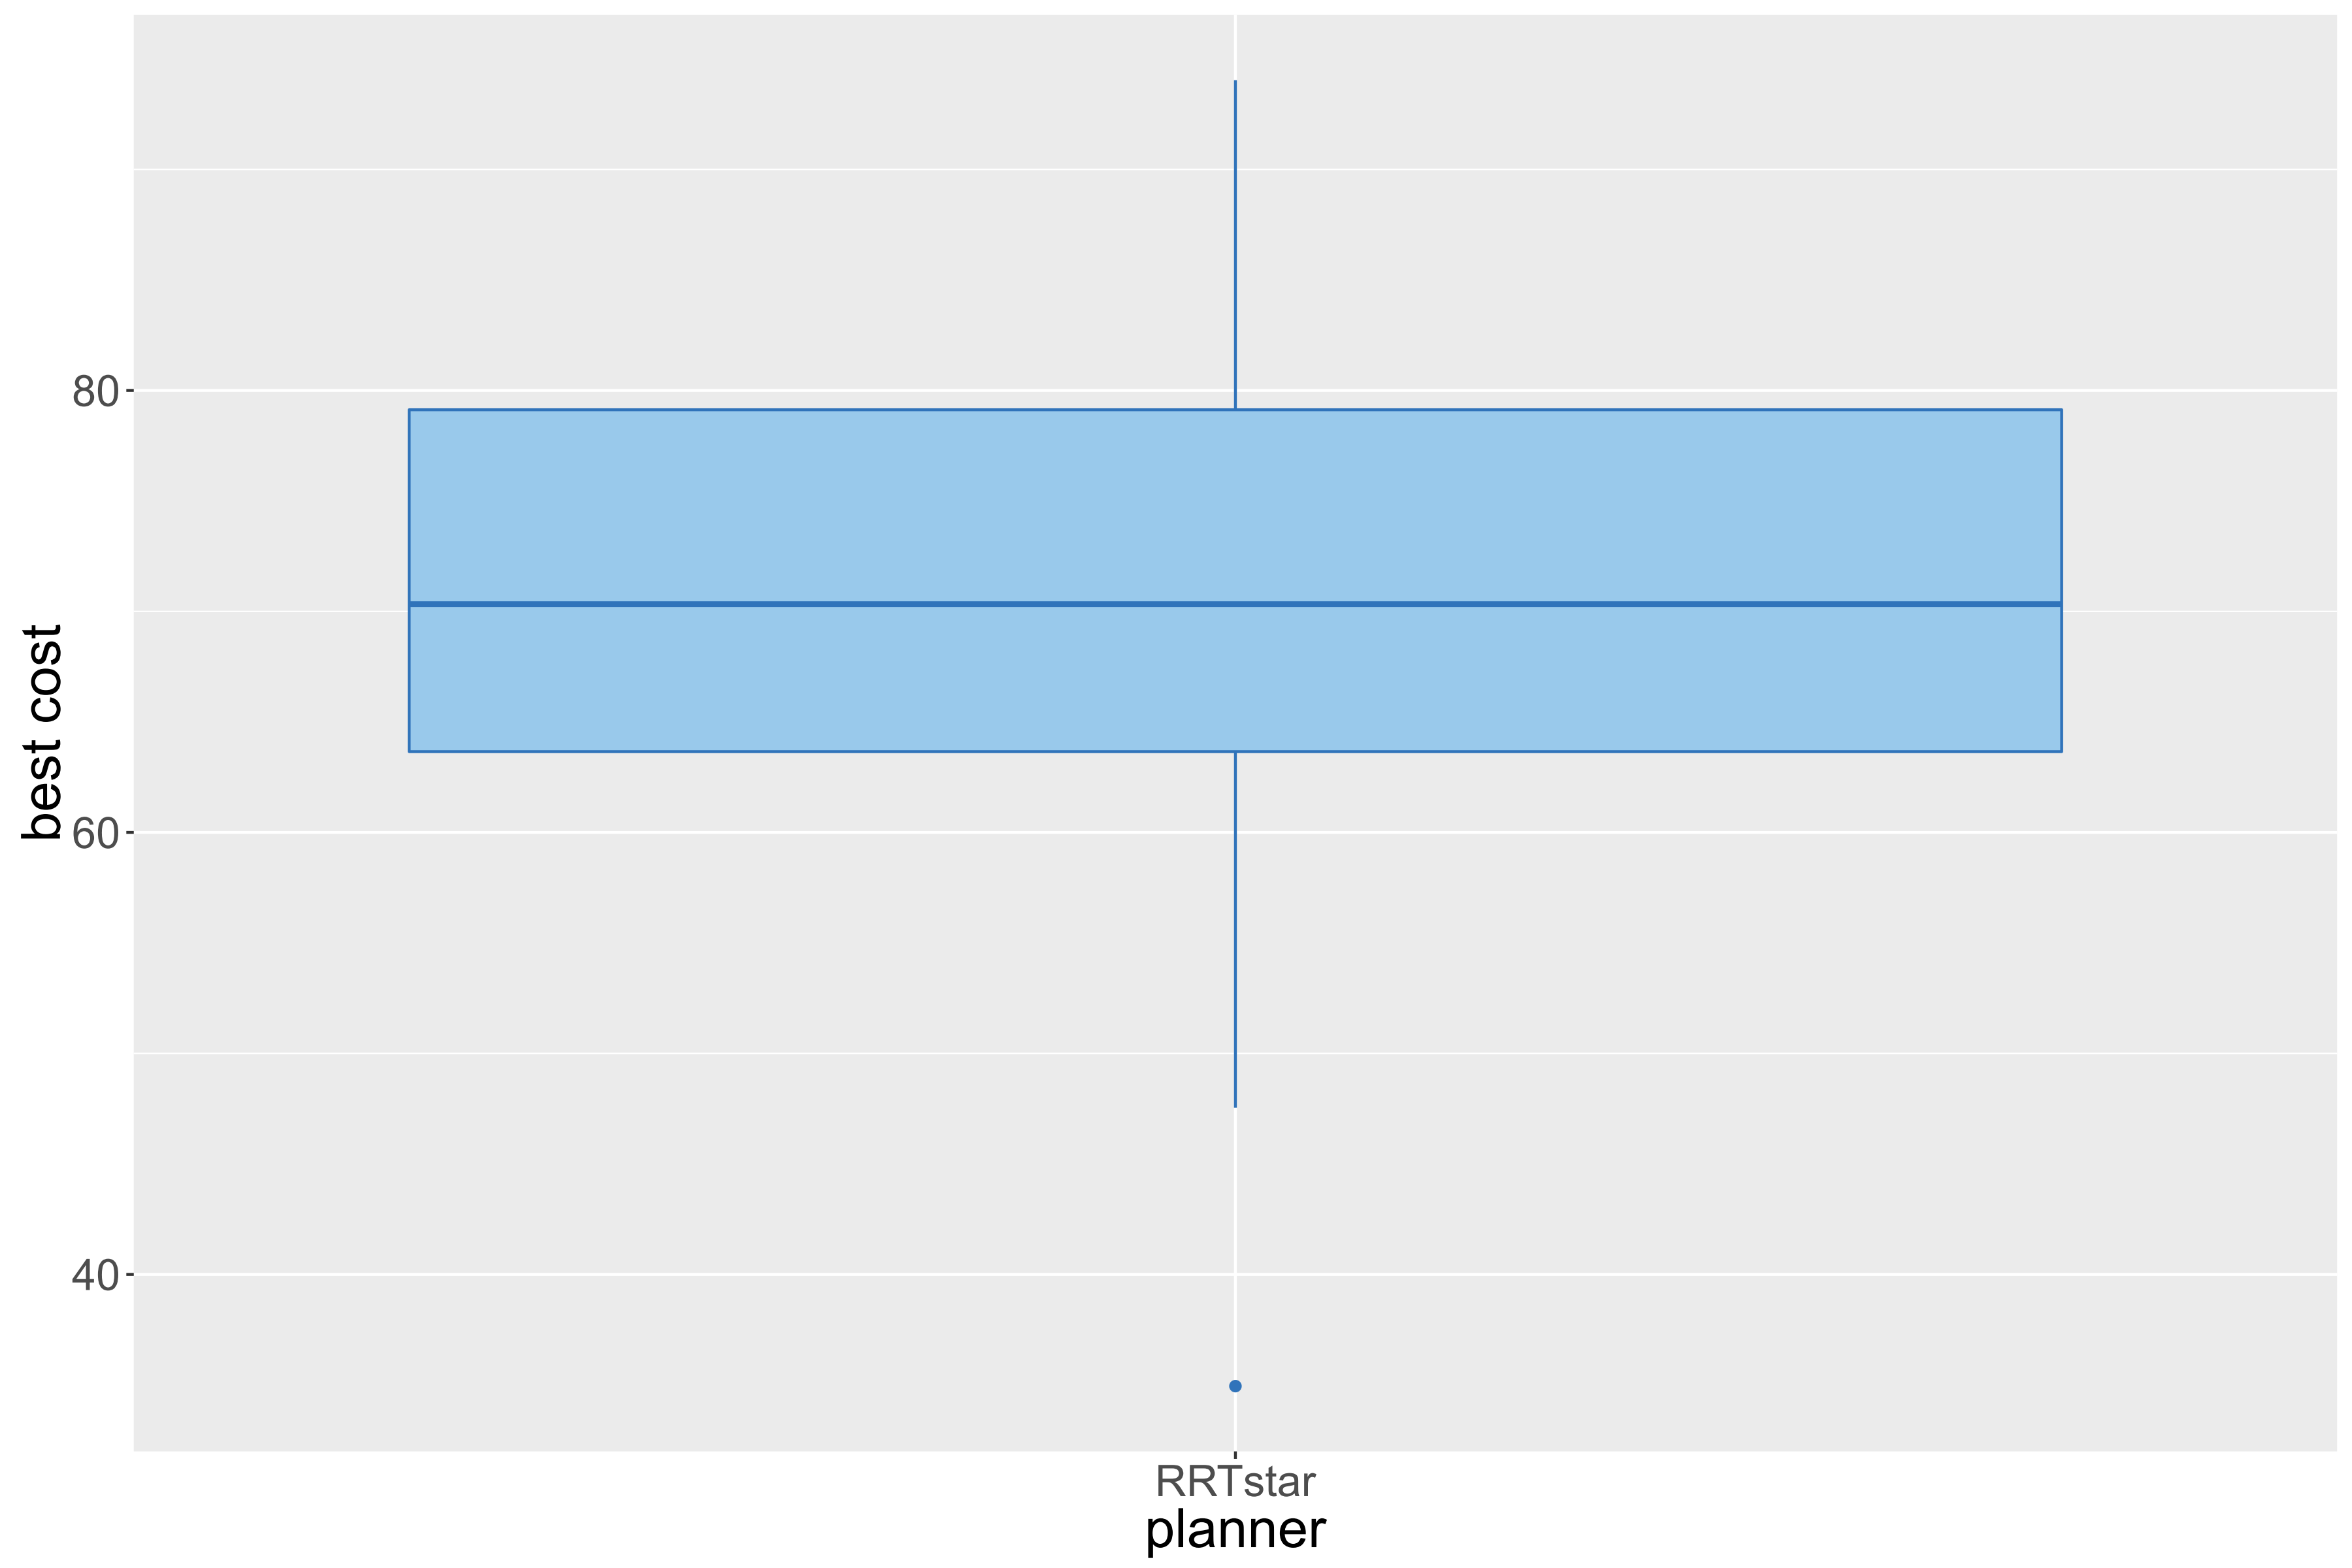
\includegraphics[width=0.8\textwidth,scale=0.6]{images/bestcost_uopt.png}}
		\caption{Best Cost of Planning Instance: Unoptimized}
		\label{fig:bc1}
	\end{subfigure}
	\begin{subfigure}[b]{0.4\textwidth}
		\frame{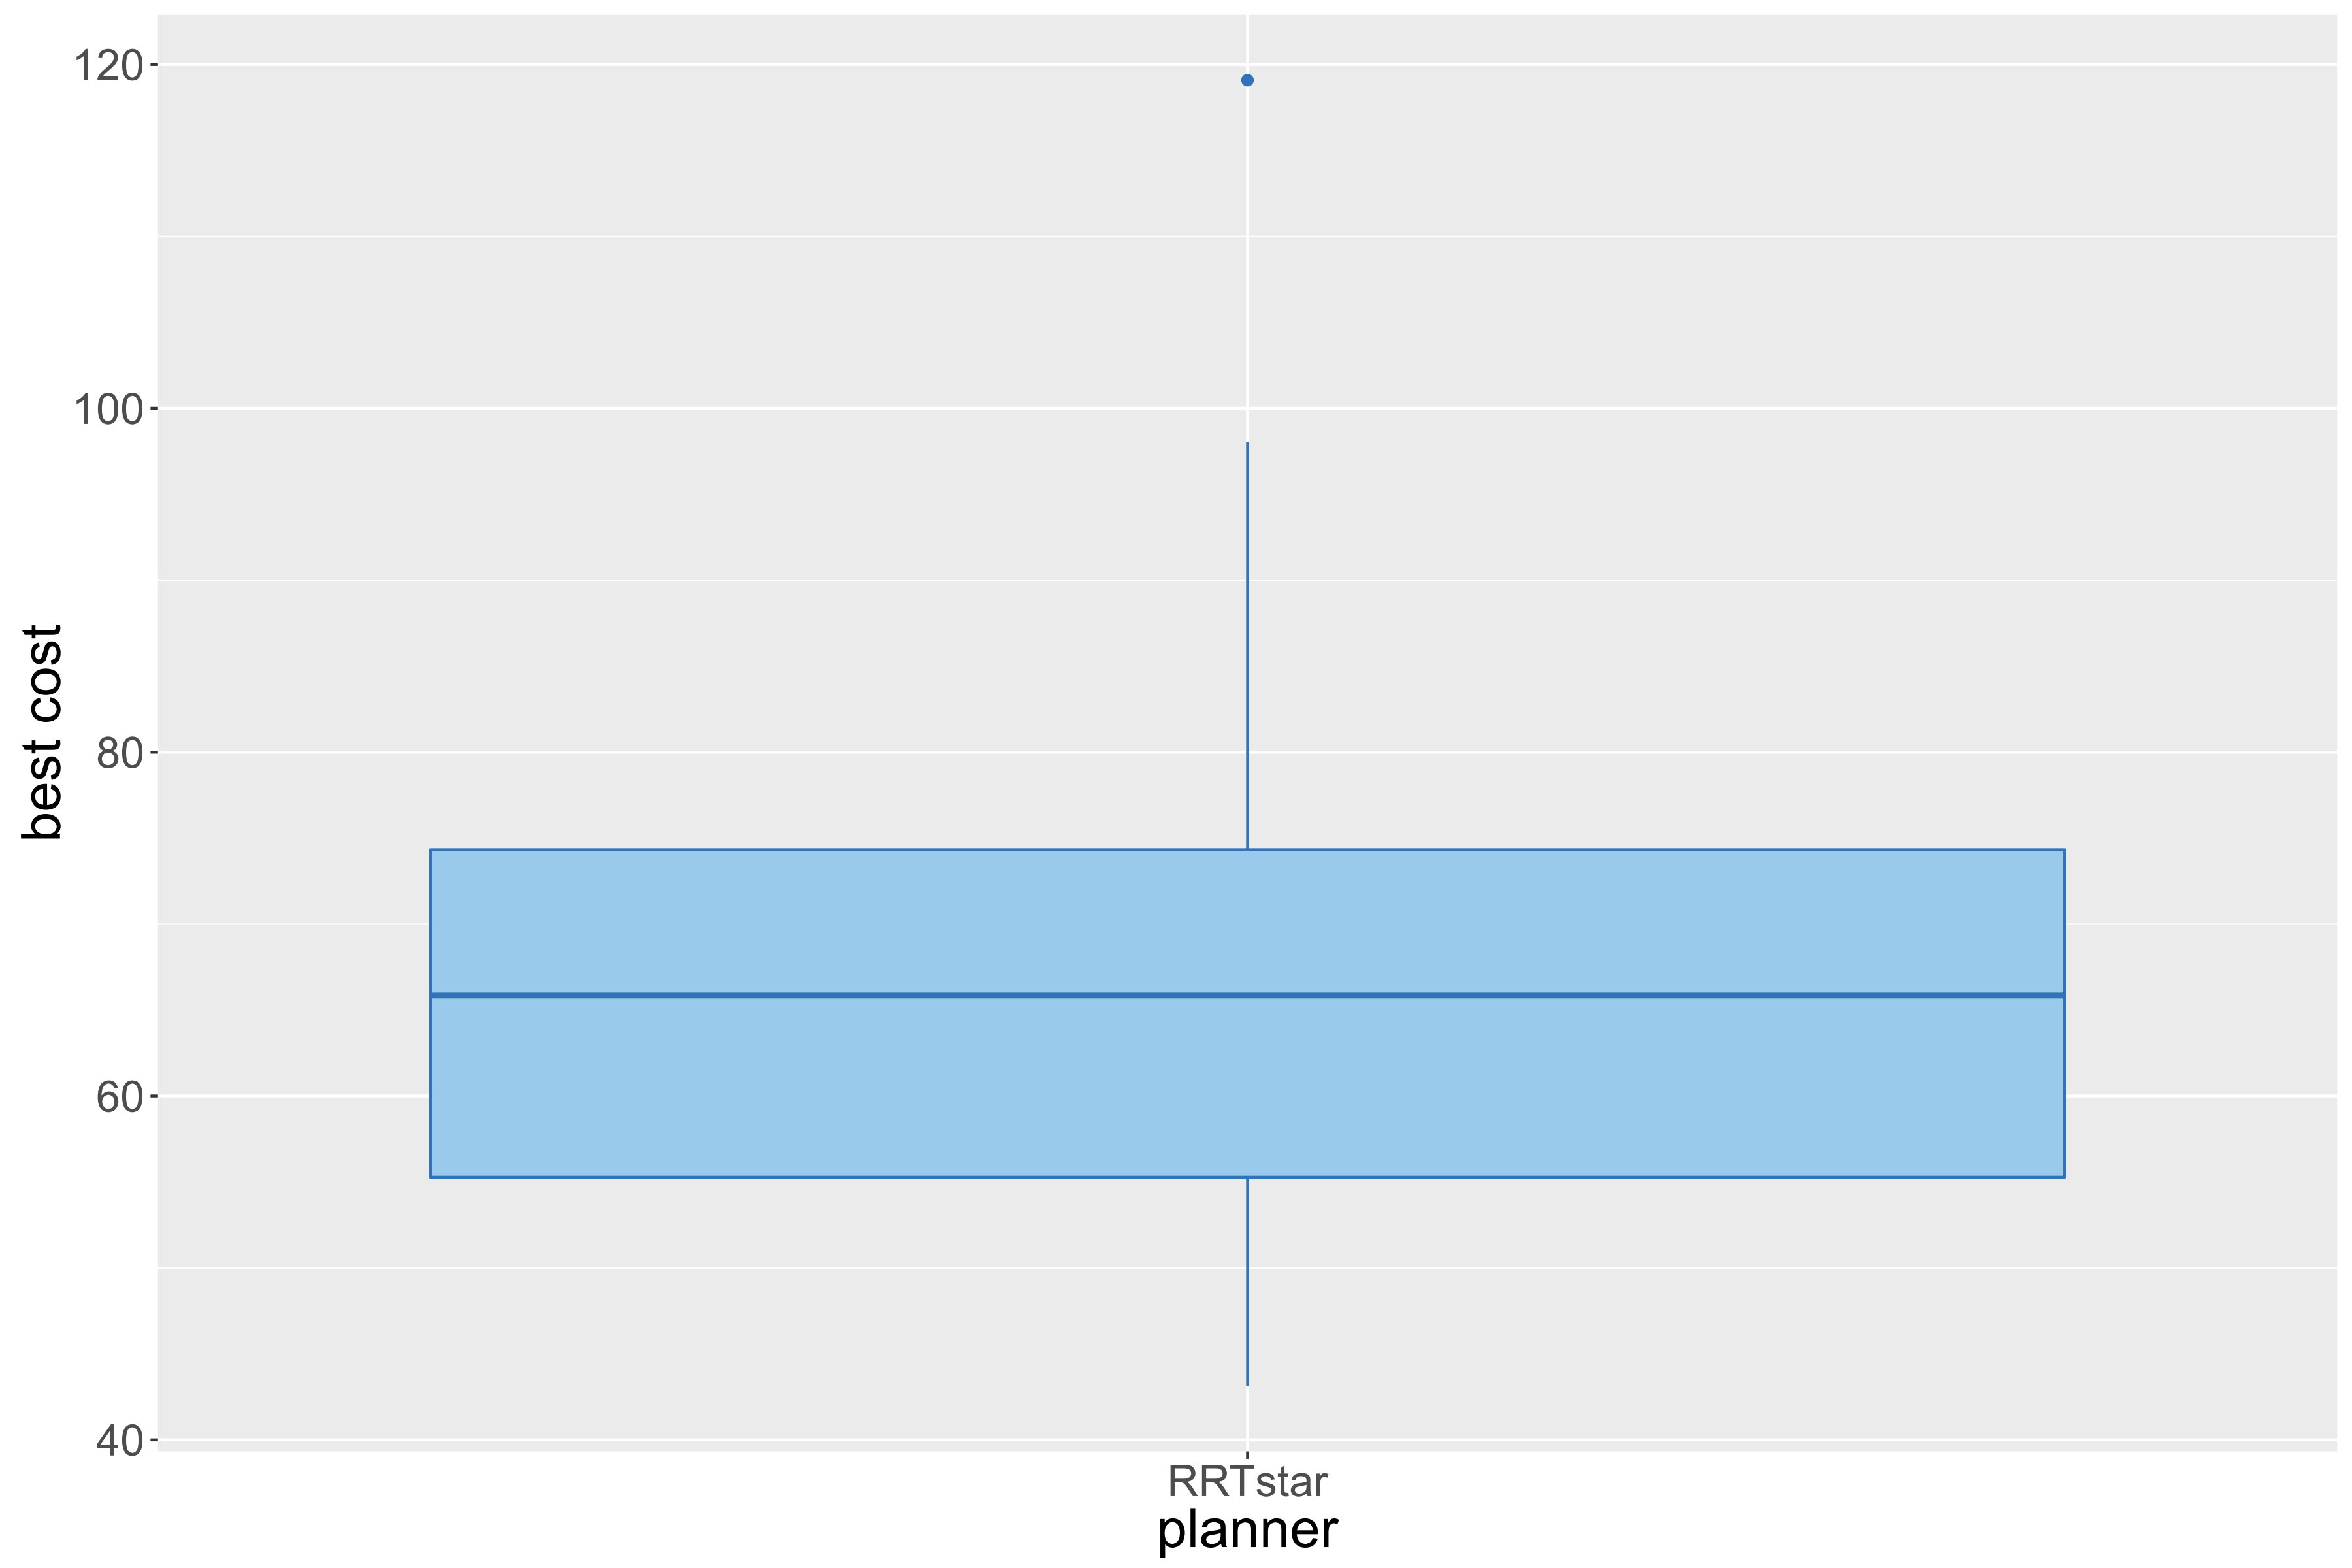
\includegraphics[width=0.8\textwidth,scale=0.6]{images/bestcost_opt.png}}
		\caption{Best Cost of Planning Instance: Using Table Optimization}
		\label{fig:bc2}
	\end{subfigure}	
	\caption{Best Cost of Planning Instance}
	\label{fig:bc}
\end{figure}

From \ref{fig:bc} we can observe that when we plan with table optimization (plot \ref{fig:bc2}), the median value of the best cost is approximately 65 whereas  when planned without table optimization (plot \ref{fig:bc1}) it is approximately 71. Even the overall range of values generated for optimized use case is lower than the range of values generated for unoptimized use case.

We next consider the case of number of graph states or samples generated by the planners while planning. Since different planners generate distinct number of samples based on their functionality, we compare the performance of each planner separately to provide a clear picture.

\begin{figure}[!htbp] %  figure placement: here, top, bottom, or page
	\centering
	\begin{subfigure}[b]{0.4\textwidth}
		\frame{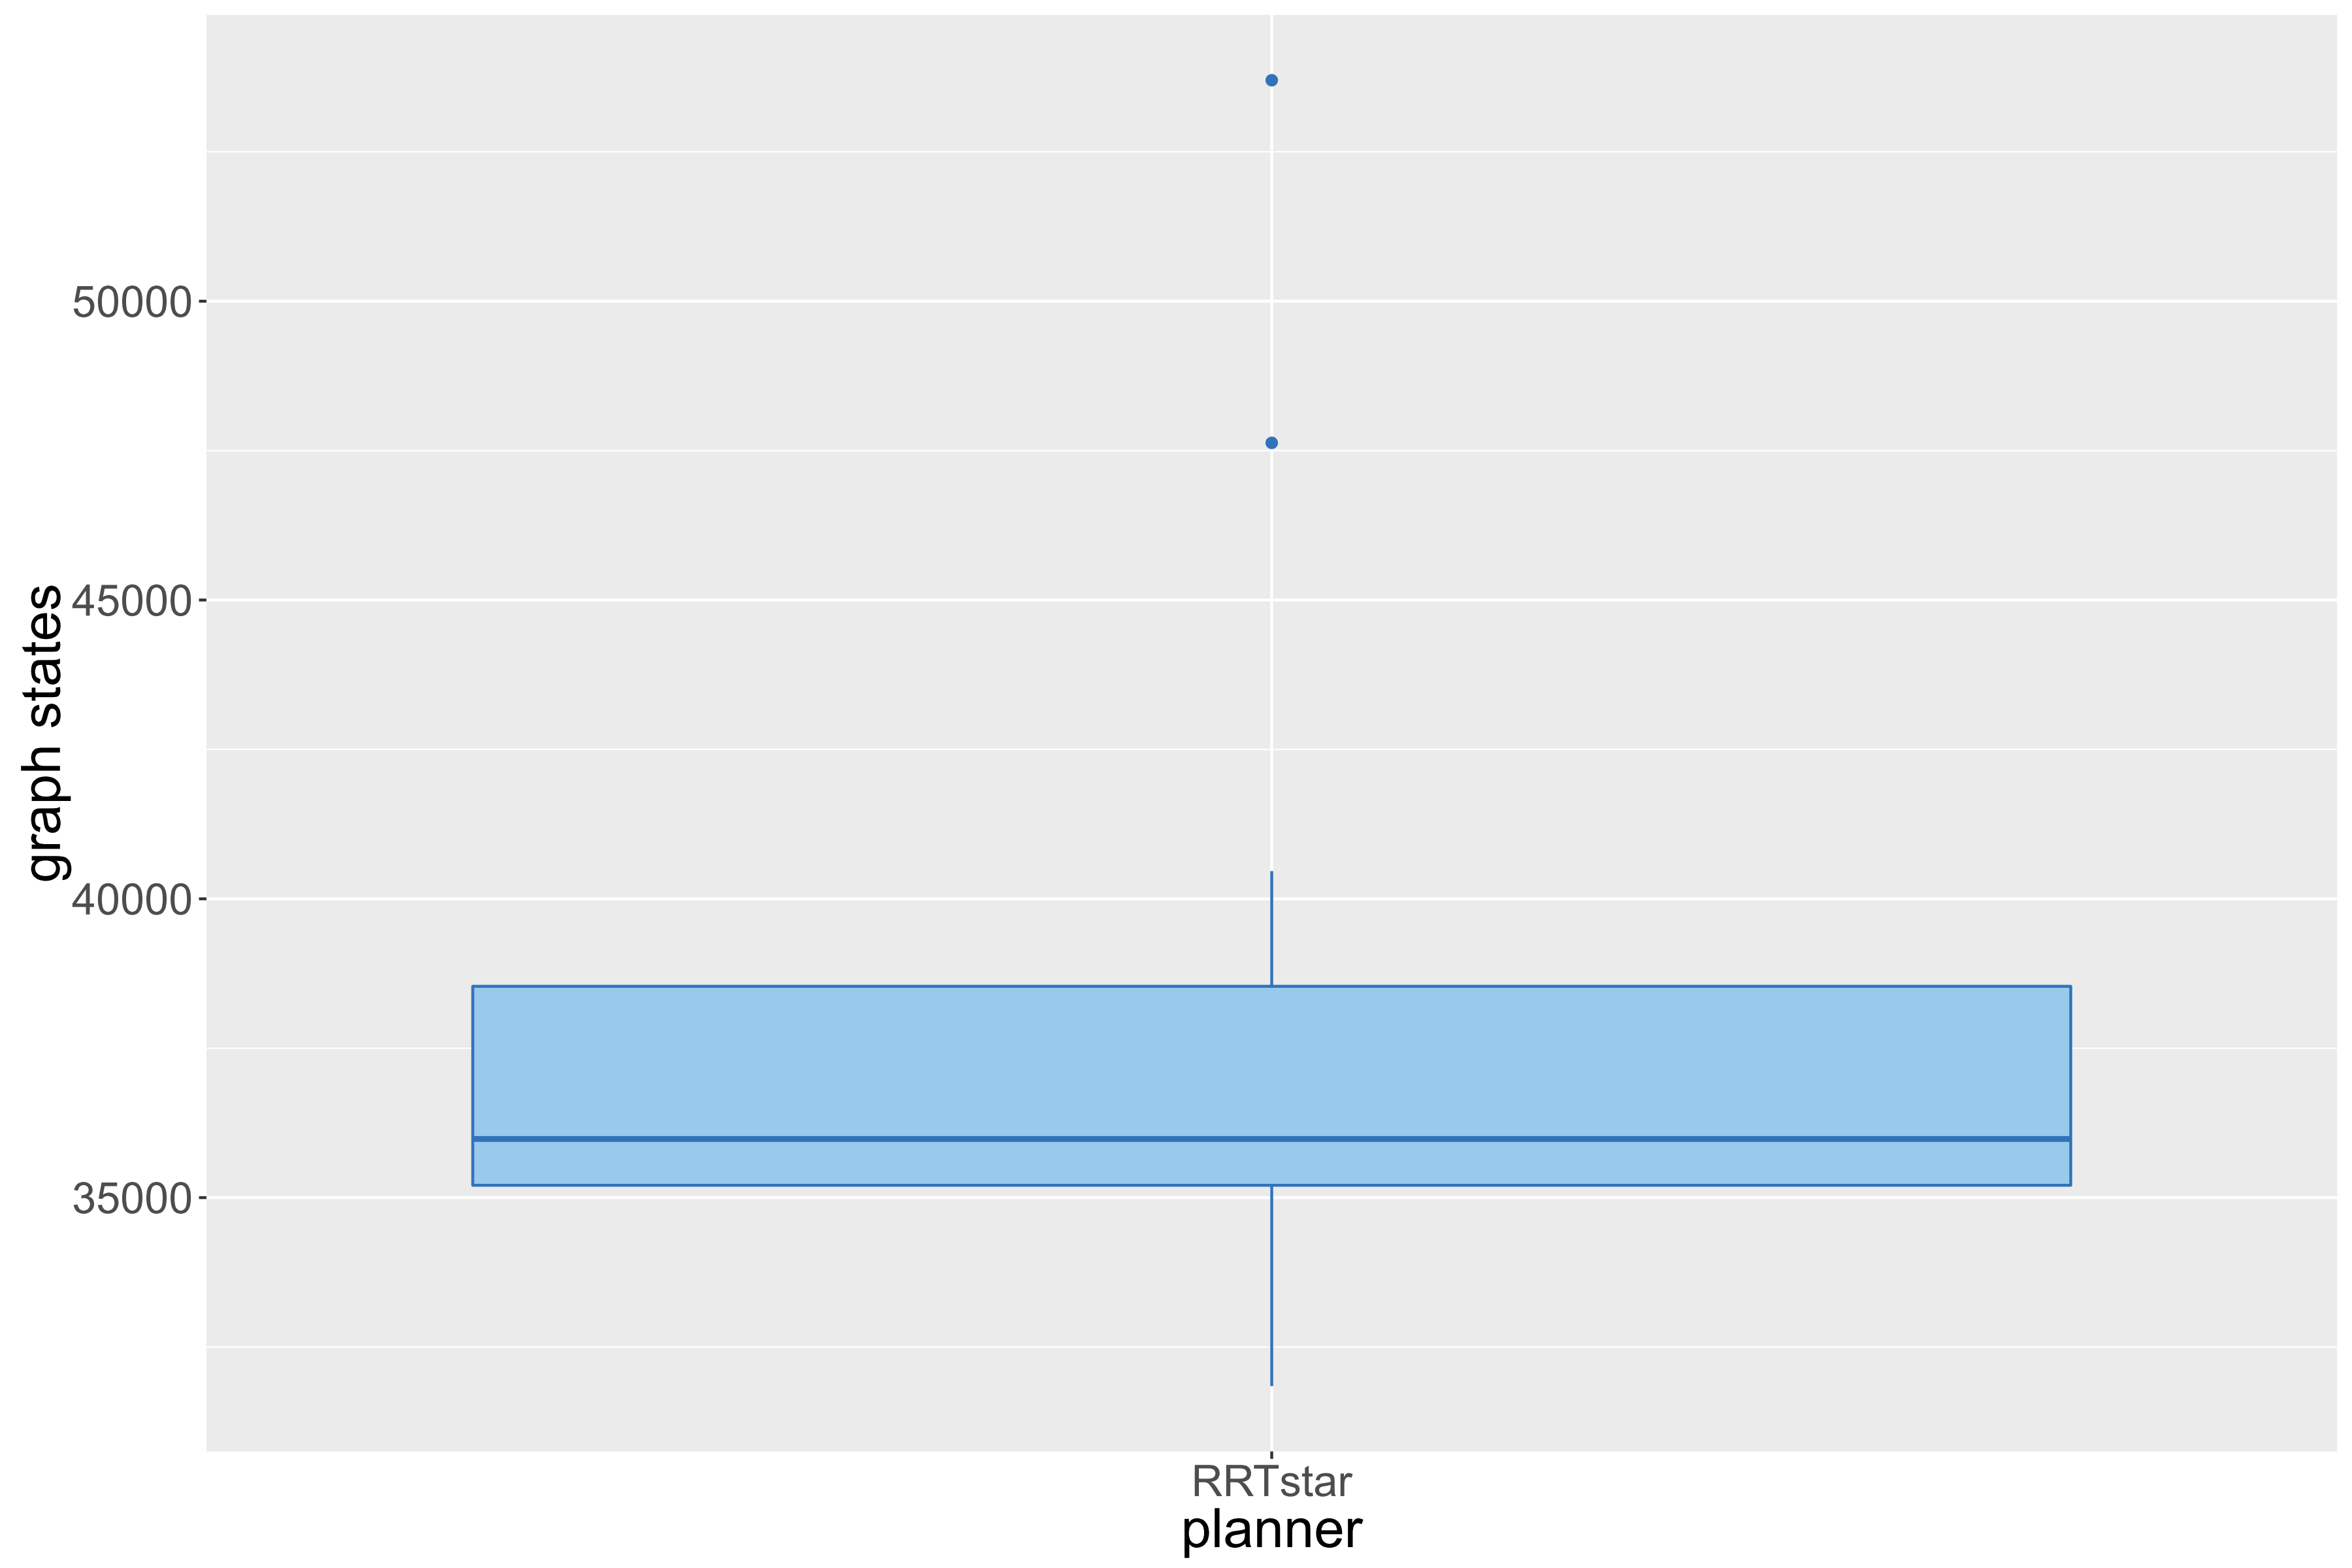
\includegraphics[width=0.8\textwidth,scale=0.6]{images/graph_state_rrt_uopt.png}}
		\caption{Number of Graph States Generated in Planning Instance: Unoptimized}
		\label{fig:gsrrt1}
	\end{subfigure}
	\begin{subfigure}[b]{0.4\textwidth}
		\frame{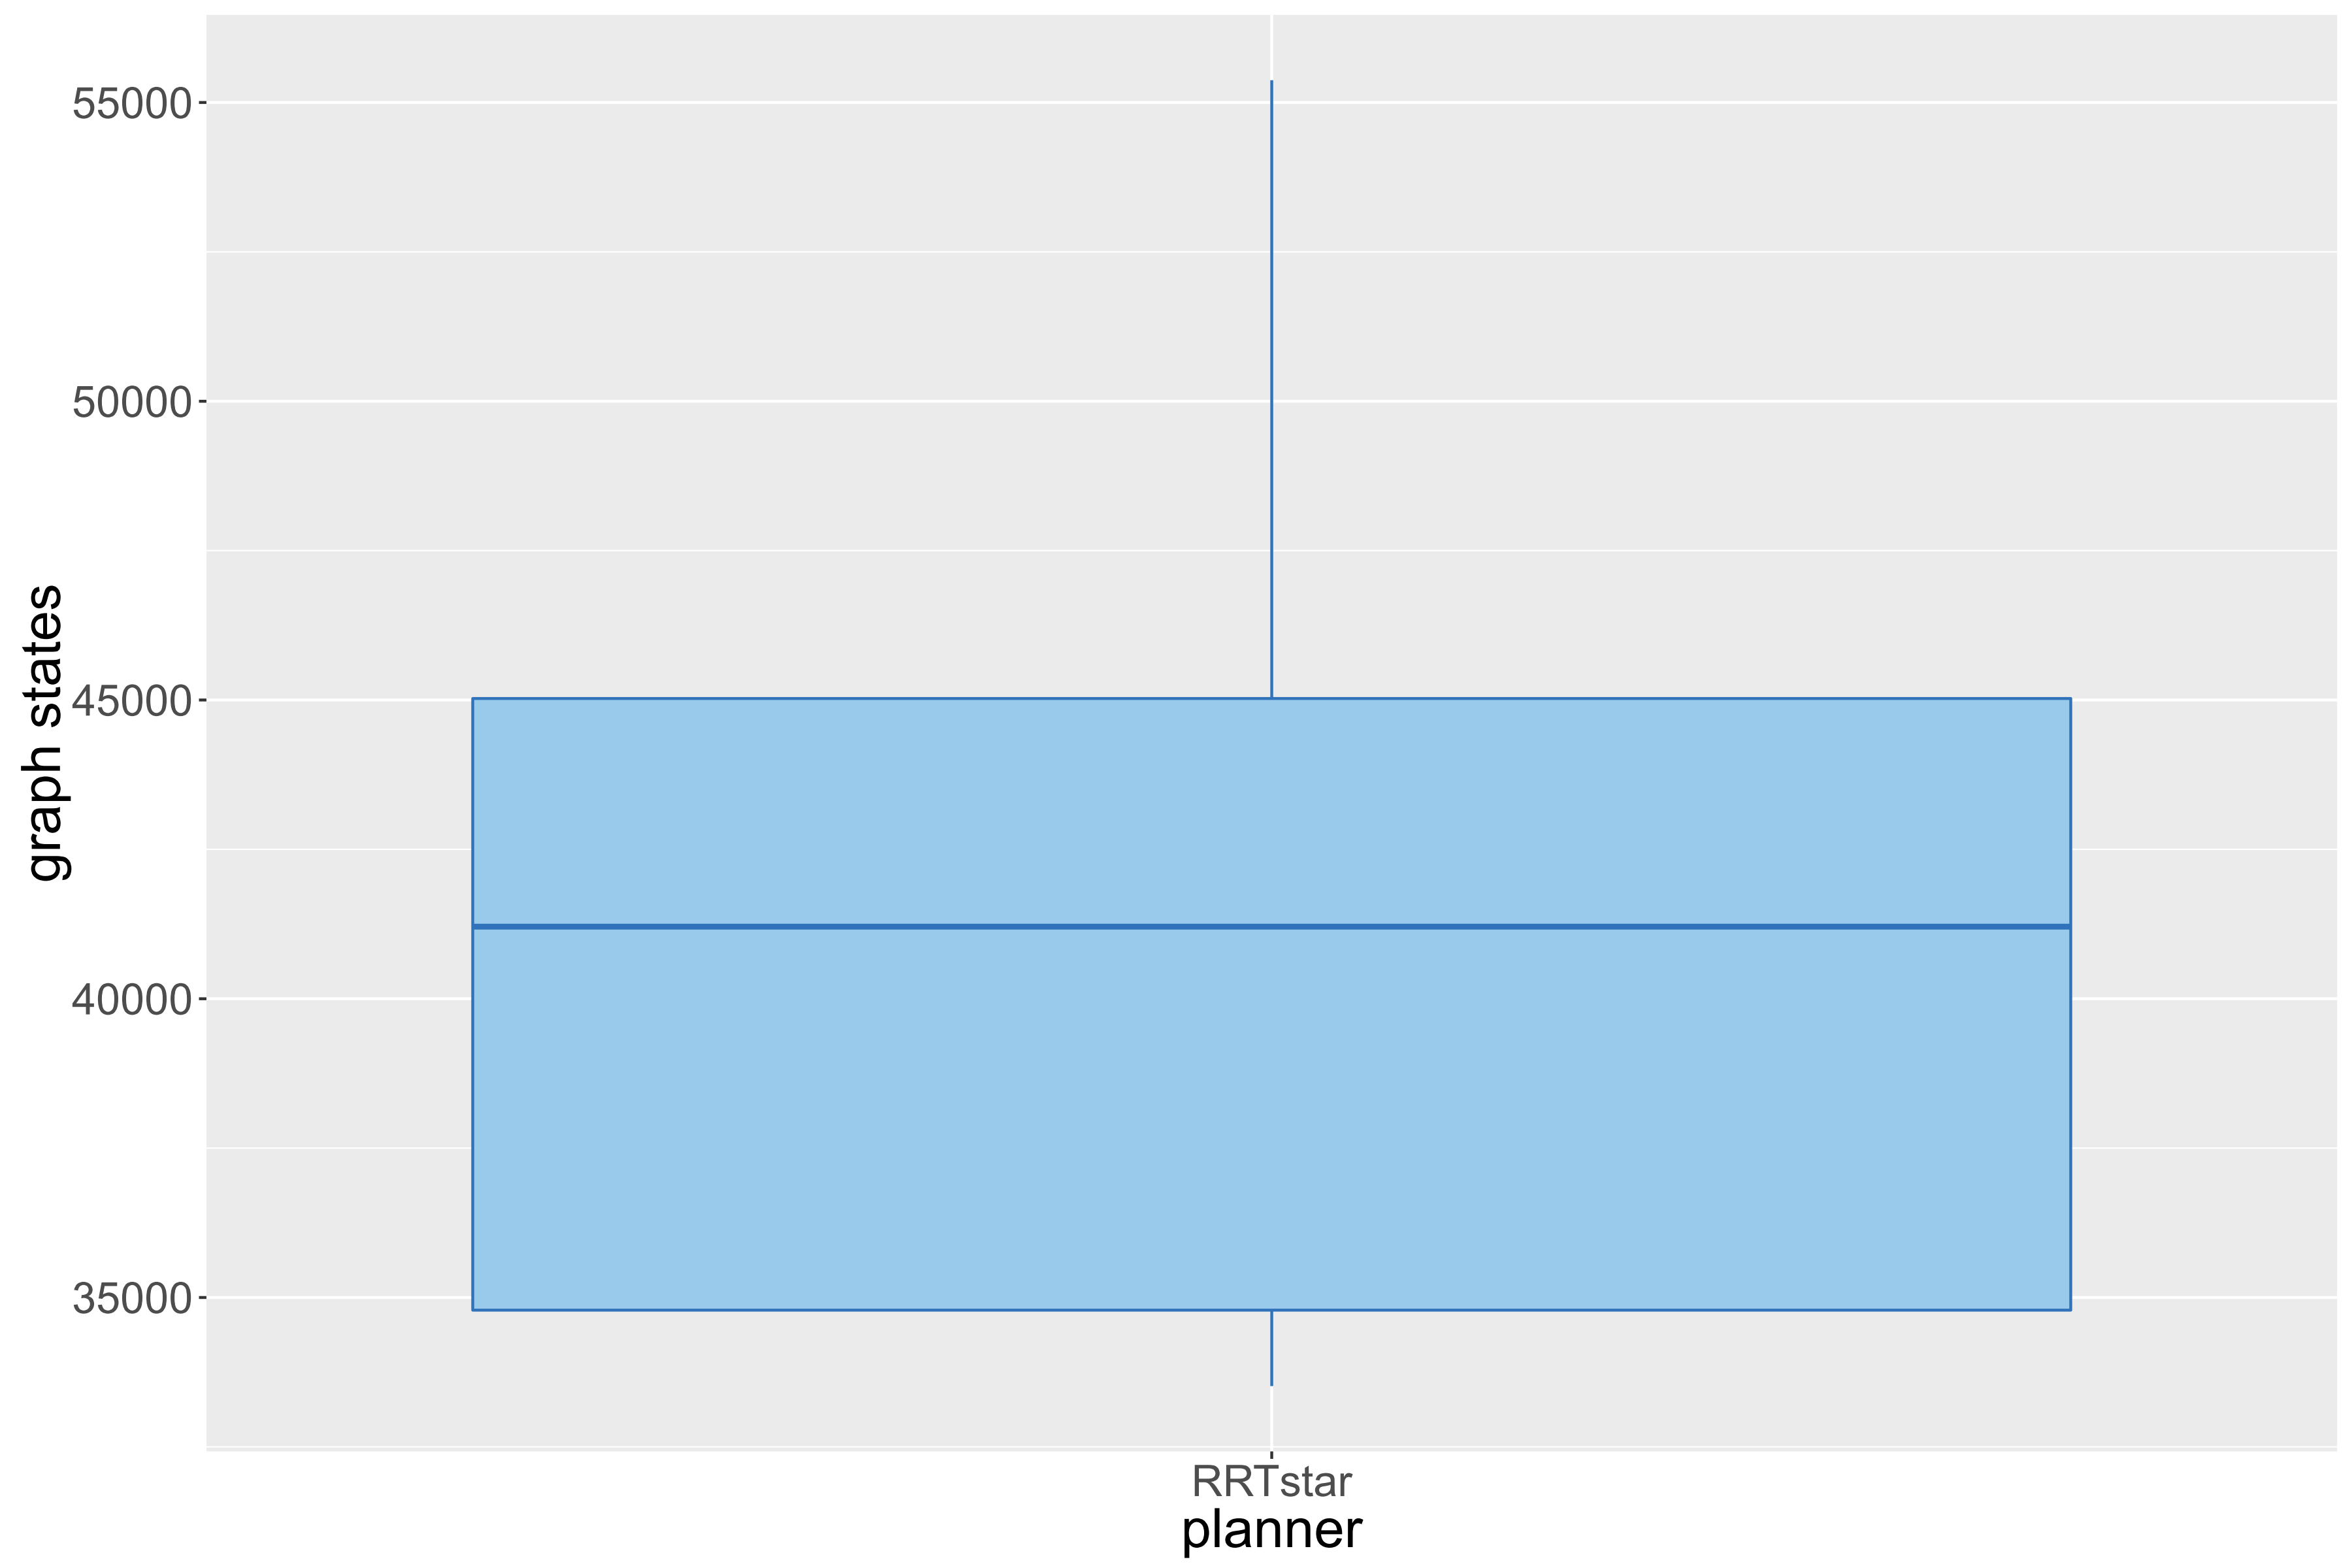
\includegraphics[width=0.8\textwidth,scale=0.6]{images/graph_state_rrt_opt.png}}
		\caption{Number of Graph States Generated in Planning Instance: Using Table Optimization}
		\label{fig:gsrrt2}
	\end{subfigure}	
	\caption{Number of Graph States Generated in Planning Instance}
	\label{fig:gsrrt}
\end{figure}

In plot (\ref{fig:bmt}), we observed that the time taken by each planner are same in both use cases. From plot (\ref{fig:gsrrt}), we can observe that the number of graph states generated by the RRT star when table optimization is used is significantly greater than the number of graph states generated by RRT star without using table optimization. If a planner generates more graph states during a planning instance while consuming the same time, it means it can cover larger part of the planning space and find out more optimal solutions. This corroborates our observation in plot \ref{fig:bc}, where we saw that for planning using table optimization the RRT star generates more solutions with better costs. 
